% Drawing 154/01-6 -- folder 154, batch 01, archive page 13 (PDF page 14).
% Transcription: figure : deux pseudo-droites orange et un faisceau issu d'un point d'une droite jaune
% Kind: pencil of pseudolines on a line. Method 2 (schematic redraw from the facsimile). Status: ok.
% Notes: Left column: three orange lines through a marked point of the yellow line, and two more orange pseudolines crossing above it. (The figure at the head of the column, with a, b, c, is described by the transcription in a \note, not by this mark.)
% Coordinates: 1 unit = 1 mm = 1/100 of the crop width (bbox in page fractions: [0.13, 0.319, 0.356, 0.4]).
% Redrawn by Claude (claude-opus-5-5), issue #73, 2026-11-07; not checked by a human; not compiled (no TeX in the session).
% Rights: reproduces part of the work -- behind RENDER_TRANSCRIPTS, never published by itself.
\documentclass[tikz,border=3pt]{standalone}
\usepackage{amsmath,amssymb}
\usetikzlibrary{patterns,arrows.meta}
\tikzset{Or/.style={orange!90!black}, Ye/.style={yellow!80!orange}, Lg/.style={green!60!black!70}, Dg/.style={green!45!black}, Br/.style={brown!80!black}, Rd/.style={red!85!black}, Bl/.style={blue!70!black}, Gy/.style={black!40}, pencil/.style={black!45}, struck/.style={black!35}, mark/.style={circle,draw,inner sep=1.3pt}, pt/.style={circle,fill,inner sep=0.9pt}, opt/.style={circle,draw,fill=white,inner sep=1.1pt}}
\begin{document}
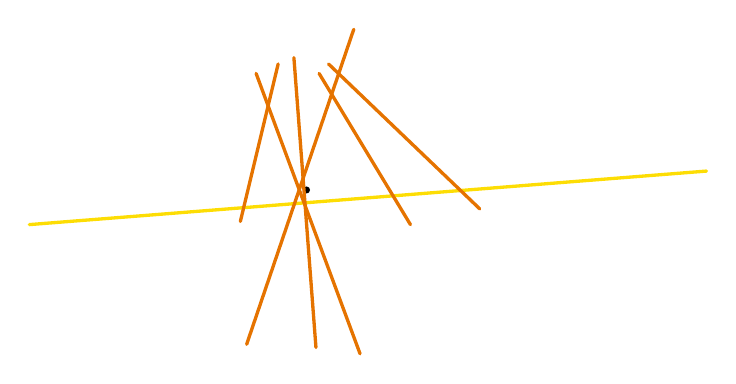
\begin{tikzpicture}[x=1mm,y=1mm,line cap=round,line join=round,font=\scriptsize]
\draw[Ye,very thick] (6.8,-29.6) -- (92.8,-22.8);
\node[pt] at (42,-25.2) {};
\draw[Or,very thick] (34.4,-44.8) -- (48,-4.8);
\draw[Or,very thick] (43.2,-45.2) -- (40.4,-8.4);
\draw[Or,very thick] (48.8,-46) -- (35.6,-10.4);
\draw[Or,very thick] (33.6,-29.2) -- (38.4,-9.2);
\draw[Or,very thick] (44.8,-9.2) -- (64,-27.6);
\draw[Or,very thick] (43.6,-10.4) -- (55.2,-29.6);
\end{tikzpicture}
\end{document}
